\documentclass[11pt]{article}
\usepackage{geometry,marginnote} % Pour passer au format A4
\geometry{hmargin=1cm, vmargin=1cm} % 

% Page et encodage
\usepackage[T1]{fontenc} % Use 8-bit encoding that has 256 glyphs
\usepackage[english,french]{babel} % Français et anglais
\usepackage[utf8]{inputenc} 

\usepackage{lmodern,numprint}
\setlength\parindent{0pt}

% Graphiques
\usepackage{graphicx,float,grffile,units}
\usepackage{tikz,pst-eucl,pst-plot,pstricks,pst-node,pstricks-add,pst-fun,pgfplots} 

% Maths et divers
\usepackage{amsmath,amsfonts,amssymb,amsthm,verbatim}
\usepackage{multicol,enumitem,url,eurosym,gensymb,tabularx}

\DeclareUnicodeCharacter{20AC}{\euro}



% Sections
\usepackage{sectsty} % Allows customizing section commands
\allsectionsfont{\centering \normalfont\scshape}

% Tête et pied de page
\usepackage{fancyhdr} \pagestyle{fancyplain} \fancyhead{} \fancyfoot{}

\renewcommand{\headrulewidth}{0pt} % Remove header underlines
\renewcommand{\footrulewidth}{0pt} % Remove footer underlines

\newcommand{\horrule}[1]{\rule{\linewidth}{#1}} % Create horizontal rule command with 1 argument of height

\newcommand{\Pointilles}[1][3]{%
  \multido{}{#1}{\makebox[\linewidth]{\dotfill}\\[\parskip]
}}

\newtheorem{Definition}{Définition}

\usepackage{siunitx}
\sisetup{
    detect-all,
    output-decimal-marker={,},
    group-minimum-digits = 3,
    group-separator={~},
    number-unit-separator={~},
    inter-unit-product={~}
}

\setlength{\columnseprule}{1pt}

\begin{document}

\textbf{Nom, Prénom :} \hspace{8cm} \textbf{Classe :} \hspace{3cm} \textbf{Date :}\\
\vspace{-0.8cm}
\begin{center}
  \textit{Bien souvent, les réponses les plus simples dans la vie sont celles qui ne nous viennent pas aussitôt à l'esprit.}  - \textbf{Stephen King}
\end{center}
\vspace{-0.8cm}

\subsection*{Définition}

\textbf{Symétrie :} \dotfill \\
\Pointilles[1]

\textbf{ex1} Tracer le symétrique des points par rapport à 0.

\begin{figure}[H]
  \centering
  
\includegraphics[width=0.5\linewidth]{5x4-symetrie/exo1.pdf}
\end{figure}

\textbf{ex2} Tracer le symétrique de la figure par rapport à O


\begin{minipage}[t]{0.50\textwidth}
\begin{figure}[H]
  \centering
  
\includegraphics[width=\linewidth]{5x4-symetrie/exo2.pdf}
\end{figure}

\begin{figure}[H]
  \centering
  
\includegraphics[width=\linewidth]{5x4-symetrie/exo3.pdf}
\end{figure}
\end{minipage}
\begin{minipage}[t]{0.50\textwidth}
\begin{figure}[H]
  \centering
  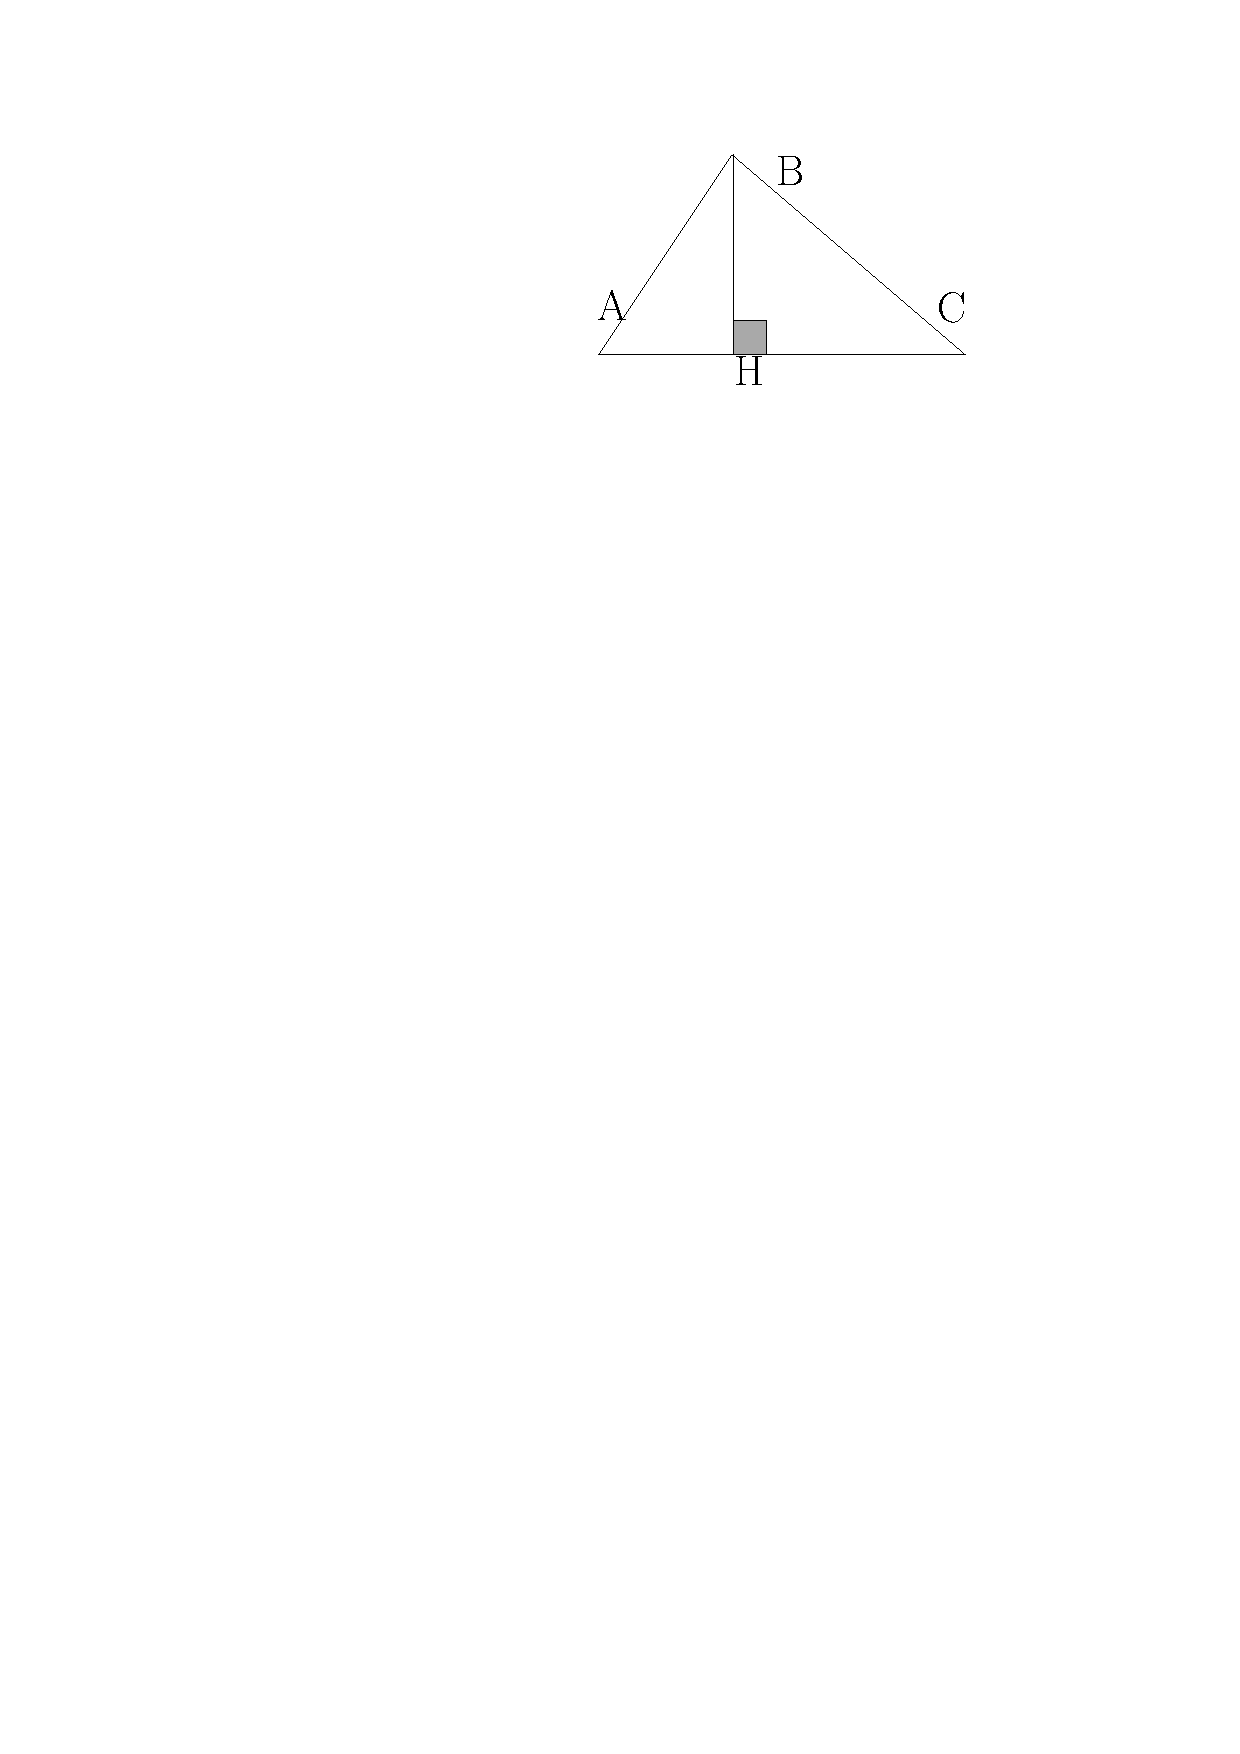
\includegraphics[width=\linewidth]{5x4-symetrie/exo4.pdf}
\end{figure}

\begin{figure}[H]
  \centering
  \includegraphics[width=\linewidth]{5x4-symetrie/exo5.pdf}
\end{figure}
\end{minipage}

\vspace{0.5cm}
\textbf{ex3} Tracer le symétrique de la figure par rapport à O

\textit{Vous devez laisser les traces de constructions}

\begin{minipage}[t]{0.50\textwidth}

\begin{figure}[H]
  \centering
  \includegraphics[width=\linewidth]{5x4-symetrie/exo6.pdf}
\end{figure}

\end{minipage}
\begin{minipage}[t]{0.50\textwidth}

\begin{figure}[H]
  \centering
  \includegraphics[width=\linewidth]{5x4-symetrie/exo7.pdf}
\end{figure}

\end{minipage}

\newpage

\textbf{ex4} Compléter la figure pour que O soit le centre de symétrie.

\begin{figure}[H]
  \centering
  \includegraphics[width=0.6\linewidth]{5x4-symetrie/exo8.pdf}
\end{figure}

\textbf{ex5} Certains logo ont un centre de symétrie. Lesquels ? Placer ces centres de symétrie.

\begin{figure}[H]
  \centering
  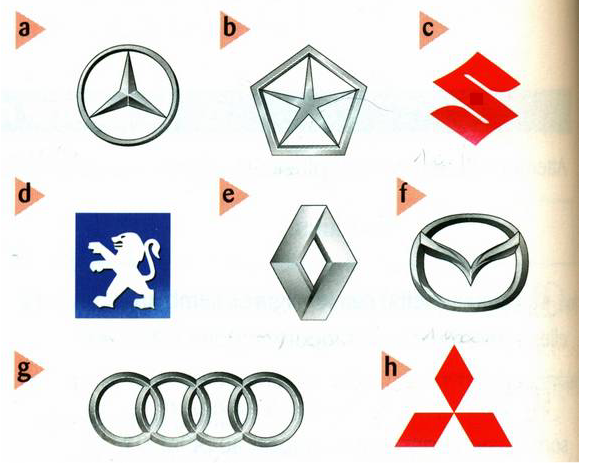
\includegraphics[width=0.6\linewidth]{5x4-symetrie/exo9.png}
\end{figure}

\textbf{Pixel Art} 

\begin{minipage}[t]{0.50\textwidth}
  \begin{figure}[H]
    \centering
    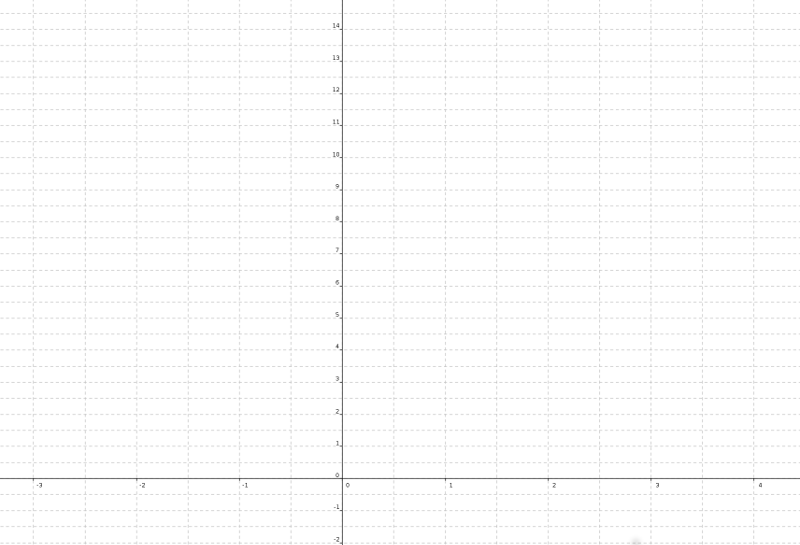
\includegraphics[width=0.8\linewidth]{5x4-symetrie/grille.png}
  \end{figure}
  \end{minipage}
  \begin{minipage}[t]{0.50\textwidth}
    \begin{figure}[H]
      \centering
      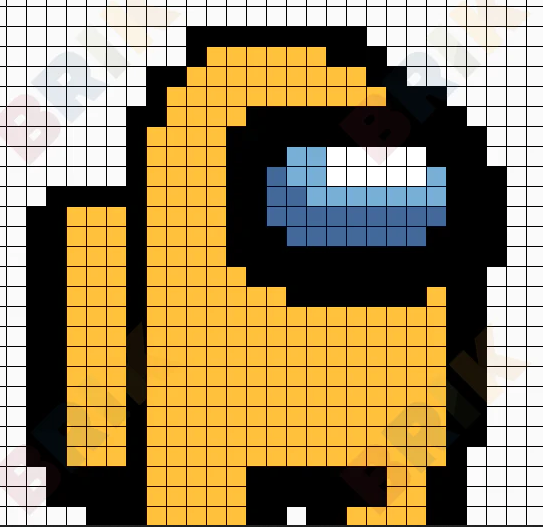
\includegraphics[width=0.8\linewidth]{5x4-symetrie/pa.png}
    \end{figure}
  \end{minipage}

\end{document}